\documentclass[dvipsnames,tikz]{standalone}
%\usepackage{xcolor}
\colorlet{tBlue}{RoyalBlue!35!Cerulean}
\colorlet{tRed}{Red}
\definecolor{tGreen}{HTML}{569909}
\definecolor{tOrange}{HTML}{FA7602}
%\usepackage{tikz}
%\usepackage{standalone}
\usetikzlibrary{decorations.pathreplacing,decorations.markings}

\tikzset{
	% style to apply some styles to each segment of a path
	on each segment/.style={
		decorate,
		decoration={
			show path construction,
			moveto code={},
			lineto code={
				\path [#1]
				(\tikzinputsegmentfirst) -- (\tikzinputsegmentlast);
			},
			curveto code={
				\path [#1] (\tikzinputsegmentfirst)
				.. controls
				(\tikzinputsegmentsupporta) and (\tikzinputsegmentsupportb)
				..
				(\tikzinputsegmentlast);
			},
			closepath code={
				\path [#1]
				(\tikzinputsegmentfirst) -- (\tikzinputsegmentlast);
			},
		},
	},
	% style to add an arrow in the middle of a path
	mid arrow/.style={postaction={decorate,decoration={
				markings,
				mark=at position .5 with {\arrow[#1]{stealth}}
	}}},
}
\begin{document}
	
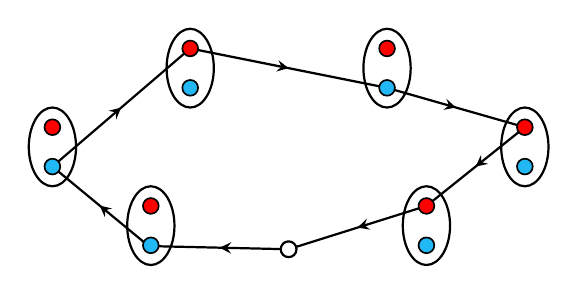
\begin{tikzpicture}
%v1=1, v2=1, v3=2, v4=2, v5=3, v6=4, v7=4, v8=5, v9=5, v10=6, v11=6, v12=6, v13=6, v14=7, v15=8, v16=9
%\draw [help lines] (0,-0.5) grid (10, 5);

%----------------------------
%Edges (clockwise)
\draw [thick,postaction={mid arrow}] (5,0.2) -- (3.25,0.24); % dummy to bottom left blue
\draw [thick,postaction={mid arrow}] (3.2,0.26) -- (2,1.25); % bottom left blue to middle left blue
\draw [thick,postaction={mid arrow}] (2,1.25) -- (3.75,2.75); % middle left blue to top left red
\draw [thick,postaction={mid arrow}] (3.75,2.75) -- (6.25,2.25); % top left red to top right blue
\draw [thick,postaction={mid arrow}] (6.25,2.25) -- (8,1.75); % top right blue to middle right red
\draw [thick,postaction={mid arrow}] (8,1.75) -- (6.75,0.75); % middle right red to bottom right red
\draw [thick,postaction={mid arrow}] (6.75,0.75) -- (5,0.2); % bottom right red to dummy

%Edges (anticlockwise)
%\draw [thick,postaction={mid arrow}] (5,0.2) -- (6.75,0.24); %dummy to bottom right blue
%\draw [thick,postaction={mid arrow}] (6.75,0.26) -- (8,1.25); % bottom right blue to middle right blue
%\draw [thick,postaction={mid arrow}] (8,1.25) -- (6.25,2.75); % middle right blue to top right red
%\draw [thick,postaction={mid arrow}] (6.25,2.75) -- (3.75,2.25); % top right red to top left blue
%\draw [thick,postaction={mid arrow}] (3.75,2.25) -- (2,1.75); % top left blue to middle left red
%\draw [thick,postaction={mid arrow}] (2,1.75) -- (3.25,0.75); % middle left red to bottom left red
%\draw [thick,postaction={mid arrow}] (3.25,0.75) -- (5,0.2); % bottom left red to dummy

\draw [thick] (3.25,0.5) ellipse (3mm and 5mm);
\draw [thick] (2,1.5) ellipse (3mm and 5mm);
\draw [thick] (3.75,2.5) ellipse (3mm and 5mm);
\draw [thick] (6.25,2.5) ellipse (3mm and 5mm);
\draw [thick] (8,1.5) ellipse (3mm and 5mm);
\draw [thick] (6.75,0.5) ellipse (3mm and 5mm);

% Vertices
\draw [fill=white, thick] (5,0.2) circle [radius = 0.1]; %dummy, vertex v_0

%Bottom left
\draw [fill=tRed, semithick] (3.25,0.75) circle [radius = 0.1]; %1 
\draw [fill=tBlue, semithick] (3.25,0.25) circle [radius = 0.1]; %2

%Middle left
\draw [fill=tRed, semithick] (2,1.75) circle [radius = 0.1]; %1
\draw [fill=tBlue, semithick] (2,1.25) circle [radius = 0.1]; %2

%Top left
\draw [fill=tRed, semithick] (3.75,2.75) circle [radius = 0.1]; %1
\draw [fill=tBlue, semithick] (3.75,2.25) circle [radius = 0.1]; %2

%Top right
\draw [fill=tRed, semithick] (6.25,2.75) circle [radius = 0.1]; %1
\draw [fill=tBlue, semithick] (6.25,2.25) circle [radius = 0.1]; %2

%Middle right
\draw [fill=tRed, semithick] (8,1.75) circle [radius = 0.1]; %1
\draw [fill=tBlue, semithick] (8,1.25) circle [radius = 0.1]; %2

%Bottom right
\draw [fill=tRed, semithick] (6.75,0.75) circle [radius = 0.1]; %1
\draw [fill=tBlue, semithick] (6.75,0.25) circle [radius = 0.1]; %2



%Edges
%\draw [thick] (5,0) -- (2.75,0.5);
%\draw [thick] (2.75,0.5) -- (1.5,2);
%\draw [thick] (1.5,2) -- (3.75,3.5);
%\draw [thick] (3.75,3.5) -- (6.25,3.5);
%\draw [thick] (6.25,3.5) -- (8,2);
%\draw [thick] (8,2) -- (6.75,0.5);
%\draw [thick] (6.75,0.5) -- (5,0);

% Vertices
%\draw [fill=white, thick] (5,0) circle [radius = 0.1]; %dummy, vertex v_0

%\draw [fill=white, thick] (2.65,0.5) circle [radius = 0.1]; %1
%\draw [fill=white, thick] (3.35,0.5) circle [radius = 0.1]; %2

%\draw [fill=white, thick] (1.4,2) circle [radius = 0.1]; %1
%\draw [fill=white, thick] (2.1,2) circle [radius = 0.1]; %2 

%\draw [fill=white, thick] (3.15,3.5) circle [radius = 0.1]; %1
%\draw [fill=white, thick] (3.85,3.5) circle [radius = 0.1]; %2

%\draw [fill=white, thick] (6.15,3.5) circle [radius = 0.1]; %1
%\draw [fill=white, thick] (6.85,3.5) circle [radius = 0.1]; %2

%\draw [fill=white, thick] (7.9,2) circle [radius = 0.1]; %1
%\draw [fill=white, thick] (8.6,2) circle [radius = 0.1]; %2

%\draw [fill=white, thick] (6.65,0.5) circle [radius = 0.1]; %1
%\draw [fill=white, thick] (7.35,0.5) circle [radius = 0.1]; %2





\end{tikzpicture}
	
\end{document}
